\section{Trig (II): Graphs and Inverses}

\subsection{Review problems}

\begin{enumerate}
\item \emph{The six basic graphs.} Match each of the graphs below to one of the six basic trig functions.
\begin{figure}[H]
\centering
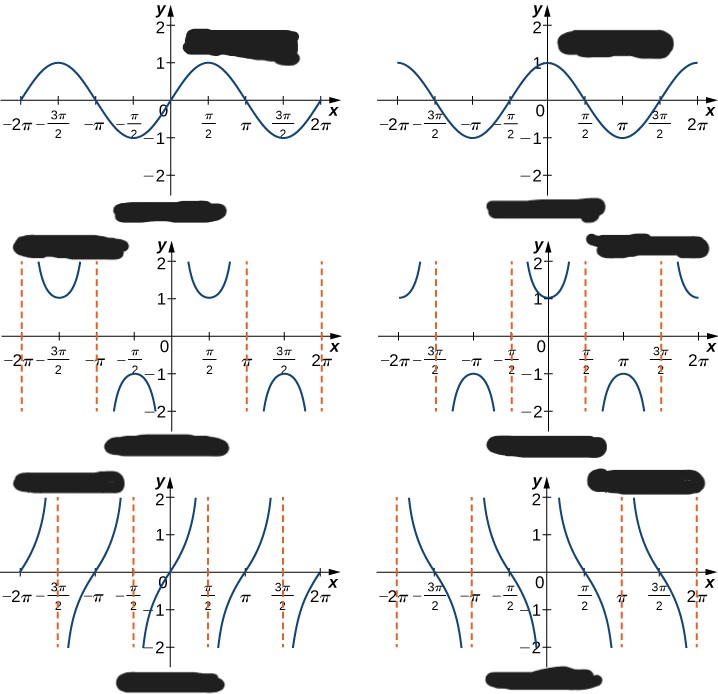
\includegraphics[scale=0.7]{img-trig-graphs.jpg}
\end{figure}
\item \emph{Period and frequency.} A function $f:\mathbb{R}\to\mathbb{R}$ is \emph{periodic} if there is a positive real number $T$ such that $f(x + T) = f(x)$ for all real $x$. The smallest such $T$, if it exists, is the \emph{period} of $f$. If $f$ is a periodic function with period $T$, the \emph{natural frequency} of $f$ is $\nu = 1/T$ while the \emph{angular frequency} of $f$ is $\omega = 2\pi/T = 2\pi\nu$. For each of the six basic trig functions, what are the period, natural frequency, and angular frequency?
\item \emph{Transformed sinusoidal waves.} For each of the following functions $\mathbb{R}\to\mathbb{R}$, find the period, amplitude, and phase shift relative to $\sin(\omega x)$, where $\omega$ is the angular frequency of the function.
\begin{enumerate}
\item $\sin x$
\item $\cos x$
\item $3\sin(5x - \tfrac{\pi}{7})$
\item $2\sin(2x) - 2\cos(2x)$
\end{enumerate}
\item \emph{Domain and range.} What are the standard domains and ranges of each of the six basic inverse trig functions ($\arcsin$, $\arccos$, etc.)?\newpage
\item \emph{Calculating inverses.}
\begin{enumerate}
\item $\arcsin(1/2)$
\item $\arccos\left(-1/\sqrt{2}\right)$
\item $\arcsin\left(-\sqrt{3}/2\right)$
\item $\arctan(-1)$
\item $\arcsin(\sin(7\pi/6))$
\item $\cos(\arccos(-1/3))$
\item $\cos(\arctan(1/2))$
\end{enumerate}
\item 
\end{enumerate}